\section{\IFRU{Предисловие}{Preface}}

\IFRU
{Здесь (будет) немного моих заметок о \gls{reverse engineering} на русском языке для начинающих, 
для тех кто хочет научиться понимать создаваемый \CCpp компиляторами код для x86 (коего, 
практически, больше всего остального) и ARM.}
{Here are some of my notes about \gls{reverse engineering} in English language for 
those beginners who would like to learn to understand x86 (which accounts for almost 
all executable software in the world) and ARM code created by \CCpp compilers.}

\IFRU{У термина ``\gls{reverse engineering}'' несколько популярных значений: 
1) исследование скомпилированных
программ; 2) сканирование трехмерной модели для последующего копирования;
3) восстановление структуры СУБД. Настоящий сборник заметок
связан с первым значением}
{There are several popular meanings of the term ``\gls{reverse engineering}'': 
1) reverse engineering of software: researching of compiled programs;
2) 3D model scanning and reworking in order to make a copy of it;
3) recreating \ac{DBMS} structure.
These notes are related to the first meaning.}

\subsection*{\IFRU{Рассмотренные темы}{Topics discussed}}

x86, ARM.

\subsection*{\IFRU{Затронутые темы}{Topics touched}}

\oracle (\ref{oracle}),
Itanium (\ref{itanium}),
\IFRU{донглы для защиты от копирования}{copy-protection dongles} (\ref{dongles}), 
LD\_PRELOAD (\ref{ld_preload}),
\IFRU{переполнение стека}{stack overflow}, 
\ac{ELF},
\IFRU{формат файла PE в win32}{win32 PE file format} (\ref{win32_pe}),
x86-64 (\ref{x86-64}),
\IFRU{критические секции}{critical sections} (\ref{critical_sections}),
\IFRU{сисколлы}{syscalls} (\ref{syscalls}), 
\ac{TLS},
\IFRU{адресно-независимый код}{position-independent code} (\ac{PIC}) (\ref{sec:PIC}), 
profile-guided optimization (\ref{PGO}),
C++ STL (\ref{cpp_STL}),
OpenMP (\ref{openmp}),
SEH (\label{sec:SEH}).

\subsection*{\IFRU{Мини-}{Mini-}\ac{FAQ}}

\newcommand{\FNURLREDDIT}{\footnote{\url{http://www.reddit.com/r/ReverseEngineering/}}}

\begin{itemize}
\item
Q: \IFRU{Нужно ли учиться понимать язык ассемблера в наше время?}
{Should one learn to understand assembly language these days?} \\
A: \IFRU{Да: ради того чтобы понимать лучше внутреннее устройство, отлаживать код лучше и быстрее.}
{Yes: in order to have deeper understanding of the internals and to debug your software better and faster.}

\item
Q: \IFRU{Нужно ли учиться писать на языке ассемблера в наше время?}
{Should one learn to write in assembly language these days?} \\
A: \IFRU{Пожалуй, нет, если только не писать низкоуровневый код для \ac{OS}.}
{Unless one writes low-level \ac{OS} code, probably no.}

\item
Q: \IFRU{Но для написания очень оптимизированных процедур?}
{But what about writing highly optimized routines?} \\
A: \IFRU{Нет, современные компиляторы \CCpp делают это лучше.}
{No, modern \CCpp compilers do this job better.}

\item
Q: \IFRU{Нужно ли знать внутреннее устройство микропроцессоров}
{Should I learn microprocessor internals}? \\
A: \IFRU{Современные}{Modern} \ac{CPU}\IFRU{ очень сложные}{-s are very complex}.
\IFRU{Если вы не собираетесь писать очень оптимизированный код
или не работаете над кодегенератором компилятора,
тогда устройство CPU можно изучать только в общих чертах}
{If you do not plan to write highly optimized code or if you do not work on compiler's code generator
then you may still learn internals in bare outlines.}
\footnote{\IFRU{Очень хороший текст на эту тему}{Very good text about it}: \cite{AgnerFog}}.
\IFRU{В то же время для понимания и анализа кода
достаточно только знать \ac{ISA}, назначения регистров, т.е., ``внешнюю'' часть \ac{CPU}, доступную
для прикладного программиста}
{At the same time, in order to understand and analyze compiled code it is enough to know
only \ac{ISA}, register's descriptions, i.e., the ``outside'' part of a \ac{CPU} that is available to
an application programmer}.

\item
Q: \IFRU{И всё-таки, зачем мне учить ассемблер}{So why should I learn assembly language anyway}? \\
A: \IFRU{В основном для лучшего понимания происходящего во время отладки и для исследования
программ без наличия исходных кодов, включая зловреды (или вредоносы)
\footnote{современные (2013) русскоязычные термины для malware}}
{Mostly to better understand what is going on while debugging and for \gls{reverse engineering} without source code, including, but not limited to, malware}.

\item
Q: \IFRU{Как можно найти работу reverse engineer-а}{How would I search for a reverse engineering job}? \\
A: \IFRU{На reddit, посвященному RE\FNURLREDDIT, время от времени бывают hiring thread}
{There are hiring threads that appear from time to time on reddit devoted to RE\FNURLREDDIT}
(\href{http://www.reddit.com/r/ReverseEngineering/comments/1hywvr/rreverseengineerings_q3_2013_hiring_thread/}{2013 Q3}, 
\href{http://www.reddit.com/r/ReverseEngineering/comments/1vui22/rreverseengineerings_2014_hiring_thread/}{2014}).
\IFRU{Посмотрите там}{Try to take a look there}.
\end{itemize}

\subsection*{\IFRU{Об авторе}{About the author}}

\begin{tabularx}{\textwidth}{ l X }

\raisebox{-\totalheight}{
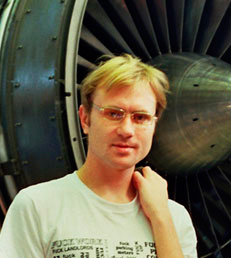
\includegraphics[scale=0.60]{Dennis_Yurichev.jpg}
}

&
\IFRU{Денис Юричев ~--- опытный reverse engineer и программист.
Также доступен как преподаватель языка ассемблера, обратной разработки (\gls{reverse engineering}), 
Си/Си++.
Может обучать удаленно через электронную почту, Skype или иной мессенджер, либо лично, в Киеве.
С его резюме можно ознакомиться на его сайте}
{Dennis Yurichev is an experienced reverse engineer and programmer.
Also available as a freelance teacher of assembly language, \gls{reverse engineering}, C/C++.
Can teach remotely via E-Mail, Skype, any other messengers, or personally in Kiev, Ukraine.
His CV is available on his website}\footnote{\url{http://yurichev.com/Dennis_Yurichev.pdf}}. \\
% FIXME: no link. \tablefootnote doesn't work
\end{tabularx}

\subsection*{\IFRU{Благодарности}{Thanks}}

\HERMIT, \IFRU{Слава ''Avid'' Казаков, Станислав ''Beaver'' Бобрицкий, Александр Лысенко, 
Александр ''Lstar'' Черненький, Андрей Зубинский, Владимир Ботов}
{Slava ''Avid'' Kazakov, Stanislav ''Beaver'' Bobrytskyy, Alexander Lysenko, 
Alexander ''Lstar'' Chernenkiy, Andrew Zubinski, Vladimir Botov}, \IFRU{Марк}{Mark} ``Logxen'' \IFRU{Купер}{Cooper},
Shell Rocket, Yuan Jochen Kang, Arnaud Patard (rtp \IFRU{на}{on} \#debian-arm IRC), 
\IFRU{и всем тем на github.com кто присылал замечания и коррективы}{and all the folks on github.com
who have contributed notes and corrections}.

\IFRU{Было использовано множество пакетов \LaTeX{}: их авторов я также хотел бы поблагодарить}
{A lot of \LaTeX{} packages were used: I would thank their authors as well}.

\subsection*{\IFRU{Отзывы об этой книге}{Praise for \IT{\TITLE}}}

\begin{itemize}
\item ``It's very well done .. and for free .. amazing.''\footnote{\url{https://twitter.com/daniel_bilar/status/436578617221742593}} Daniel Bilar, Siege Technologies, LLC.

\item ``...excellent and free''\footnote{\url{https://twitter.com/petefinnigan/status/400551705797869568}} Pete Finnigan, \RU{гуру по безопасности }\oracle\EN{ security guru}.

\item ``... book is interesting, great job!'' Michael Sikorski, \IFRU{автор книги}{author of} \IT{Practical Malware Analysis: The Hands-On Guide to Dissecting Malicious Software}.

\item ``... my compliments for the very nice tutorial!'' Herbert Bos, \IFRU{профессор университета}{full professor at the} Vrije Universiteit Amsterdam.

\item ``... It is amazing and unbelievable.'' Luis Rocha, CISSP / ISSAP, Technical Manager, Network \& Information Security at Verizon Business.

\item ``Thanks for the great work and your book.'' Joris van de Vis, SAP Netweaver \& Security specialist.

\end{itemize}

\subsection{\RU{Пожертвования}\EN{Donate}}
\label{sec:donate}

\RU{Как выясняется, быть (техническим) писателем требует много сил и работы}
\EN{As it turns out, (technical) writing takes a lot of effort and work}.

\RU{Эта книга является свободной, находится в свободном доступе, и доступна в виде исходных кодов}
\EN{This book is free, available freely and available in source code form}
\footnote{\href{http://go.yurichev.com/17089}{GitHub}} (LaTeX), 
\RU{и всегда будет оставаться таковой}\EN{and it will be so forever}.

\EN{It's also ad-free}\RU{Тут также нет рекламы}.

\RU{В мои текущие планы насчет этой книги входит добавление информации на эти темы}
\EN{My current plan for this book is to add lots of information about}:
PLANS\footnote{\href{http://go.yurichev.com/17090}{GitHub}}.

\RU{Если вы хотите, чтобы я продолжал свою работу и писал на эти темы,
вы можете рассмотреть идею пожертвования}
\EN{If you want me to continue writing on all these topics you may consider donating}.

\RU{Я писал эту книгу более года}\EN{I worked more than a year on this book}
\footnote{\RU{Самый первый коммит в git от марта 2013}\EN{Initial git commit from March 2013}: \\
\href{http://go.yurichev.com/17091}{GitHub}},
\RU{здесь более 800 страниц}\EN{there are more than 800 pages}.
\RU{Здесь как минимум $\approx 400$ \TeX-файлов, $\approx 150$ исходников на \CCpp, 
$\approx 470$ различных листингов, $\approx 160$ скриншотов}
\EN{There are at least $\approx 400$ \TeX-files, $\approx 150$ \CCpp source codes, 
$\approx 470$ various listings, $\approx 160$ screenshots}.

\RU{Цены на другие книги по этой же тематике на amazon.com колеблются в пределах от \$20 до \$50}
\EN{Price of other books on the same subject varies between \$20 and \$50 on amazon.com}.

\RU{Со способами пожертвовать деньги можно ознакомиться на странице}
\EN{Ways to donate are available on the page:} \href{http://go.yurichev.com/17011}{beginners.re}.

\RU{Имена всех жертвователей будут перечислены в книге}
\EN{Every donor's name will be included in the book}!
\RU{Жертвователи также имеют право просить меня дописывать в книгу что-то раньше, чем остальное}
\EN{Donors also have a right to ask me to rearrange items in my writing plan}.

\iffalse
\RU{Почему не попробовать издаться}\EN{Why not try to publish}?
\RU{Потому что это техническая литература, которая, как мне кажется,
не может быть закончена или быть замороженной в бумажном виде}
\EN{Because it's technical literature which, as I believe, cannot be finished or frozen in paper state}.
\RU{Такие технические справочники чем-то похожи на Wikipedia или библиотеку \ac{MSDN},
они могут развиваться бесконечно долго}
\EN{Such technical references akin to Wikipedia or \ac{MSDN} library.
They can evolve and grow indefinitely}.
\RU{Кто-то может сесть и, не отрываясь, написать всё от начала до конца, опубликовать это и забыть}
\EN{Someone can sit down and write everything from the begin to the end, publish it and forget about it}.
\RU{Как выясняется, это не я}\EN{As it turns out, it's not me}.
\RU{Каждый день меня посещают мысли вроде ``это было написано плохо, можно было бы и лучше написать'',
``это плохой пример, я знаю получше'',
``ещё одна вещь, которую я могу объяснить лучше и короче'' и т.д}
\EN{I have everyday thoughts like ``that was written badly and can be rewritten better'', 
``that was a bad example, I know a better one'', 
``that is also a thing I can explain better and shorter'', etc}.
\RU{Как можно увидеть в истории коммитов исходников этой книги,
я делаю много мелких изменений почти каждый день}
\EN{As you may see in commit history of this book's source code,
I make a lot of small changes almost every day}:
\href{http://go.yurichev.com/17092}{GitHub}.

\RU{Так что книга, наверное, будет в виде ``rolling release'', как говорят о дистрибутивах Linux вроде
Gentoo}
\EN{So the book will probably be a ``rolling release'' as they say about Linux distros like Gentoo}.
\RU{Без релизов (и дедлайнов) вообще, а постепенная разработка}
\EN{No fixed releases (and deadlines) at all, but continuous development}.
\RU{Я не знаю, сколько займет времени написать всё что я знаю. Может быть, 10 лет или больше}
\EN{I don't know how long it will take to write all I know. Maybe 10 years or more}.
\RU{Конечно, это не очень удобно для читателей, желающих стабильности,
но всё что я могу им предложить ~--- это файл ChangeLog}
\EN{Of course, it is not very convenient for readers who want something stable,
but all I can offer is a ChangeLog}
\footnote{\href{http://go.yurichev.com/17093}{GitHub}}
\RU{, служащий как секция ``что нового''}\EN{ file serving as a ``what's new'' section}.
\RU{Те, кому интересно, могут проверять его время от времени, или мой блог/twitter/facebook
\footnote{
\href{http://go.yurichev.com/17094}{blog.yurichev.com}
\href{http://go.yurichev.com/17021}{twitter}
\href{http://go.yurichev.com/17022}{facebook}
}}
\EN{Those who are interested may check it from time to time, or my blog/twitter/facebook
\footnote{
\href{http://go.yurichev.com/17094}{blog.yurichev.com}
\href{http://go.yurichev.com/17021}{twitter}
\href{http://go.yurichev.com/17022}{facebook}
}}.
\fi
\subsubsection*{\RU{Жертвователи}\EN{Donors}}

17 * \RU{аноним}\EN{anonymous}, 
2 * \RU{Олег Выговский}\EN{Oleg Vygovsky} (50+100 UAH), 
Daniel Bilar (\$50), 
James Truscott (\$4.5),
Luis Rocha (\$63), 
Joris van de Vis (\$127), 
Richard S Shultz (\$20), 
Jang Minchang (\$20), 
Shade Atlas (5 AUD), 
Yao Xiao (\$10),
Pawel Szczur (40 CHF), 
Justin Simms (\$20), 
Shawn the R0ck (\$27), 
Ki Chan Ahn (\$50), 
Triop AB (100 SEK), 
Ange Albertini (10 EUR),
\RU{Сергей Лукьянов}\EN{Sergey Lukianov} (300 RUR), 
Ludvig Gislason (200 SEK), 
Gérard Labadie (40 EUR), 
Sergey Volchkov (10 AUD),
Vankayala Vigneswararao (\$50),
Philippe Teuwen (\$4),
Martin Haeberli (\$10),
Victor Cazacov (5 EUR),
Tobias Sturzenegger (10 CHF),
Sonny Thai (\$15),
Bayna AlZaabi (\$75),
Redfive B.V. (25 EUR),
Joona Oskari Heikkilä (5 EUR),
Marshall Bishop (\$50),
Nicolas Werner (12 EUR),
Jeremy Brown (\$100),
Alexandre Borges (\$25),
Vladimir Dikovski (50 EUR),
Jiarui Hong (100.00 SEK).



\subsection*{\IFRU{Об иллюстрациях}{About illustrations}}

\IFRU{Читатели, привыкшие читать интернет-страницы, вероятно привыкли к тому что иллюстрации
находятся там же, где и должны}{Those readers who are used to read a lot in the Internet, expects
seeing illustrations at the places where they should be}.
\IFRU{Это потому что там нет разбивок на страницы, там она только одна}{It's because there 
are no pages at all, only single one}.
\IFRU{В книгах же, иллюстрации далеко не всегда удается вставить в том контексте где нужно}
{It's not possible to place illustrations in the book at the suitable context}.
\IFRU{Так что, здесь бывает так, что они все находятся в конце секции,
и по тексту на них ставятся ссылки вроде}{So, in this book, illustrations can be at the end of section,
and a referenceses in the text may be present, like}
``\figname{}1.1''.

% {\IFRU{Целевая аудитория}{Target audience}}

